\documentclass[11pt,a4paper]{article}
\usepackage[margin=18mm]{geometry}
\usepackage{amsmath,amssymb,mathtools}
\usepackage{booktabs,array,enumitem}
\usepackage[dvipsnames]{xcolor}
\usepackage{graphicx,listings,tikz,float,needspace}
\usetikzlibrary{arrows.meta,positioning}
\usepackage[most]{tcolorbox}
\usepackage{hyperref}
\hypersetup{colorlinks=true,urlcolor=MidnightBlue,linkcolor=MidnightBlue}
\setlength{\parindent}{0pt}\setlength{\parskip}{4pt}
\newcommand{\course}{PHY4605 Computational Methods in Physics}
\newcommand{\units}[1]{\,\mathrm{#1}}
\newtcolorbox{keybox}{colback=RoyalBlue!5,colframe=RoyalBlue!65!black,boxrule=.7pt,arc=2mm}
\newtcolorbox{checkbox}{colback=ForestGreen!5,colframe=ForestGreen!55!black,boxrule=.7pt,arc=2mm}
\newtcolorbox{aibox}{colback=BurntOrange!7,colframe=BurntOrange!80!black,boxrule=.7pt,arc=2mm}
\lstdefinestyle{matlabstyle}{language=Matlab,basicstyle=\ttfamily\footnotesize,keywordstyle=\color{RoyalBlue!75!black},commentstyle=\color{ForestGreen!55!black},stringstyle=\color{BurntOrange!80!black},numbers=left,numberstyle=\scriptsize\color{black!50},numbersep=5pt,frame=single,rulecolor=\color{RoyalBlue!25},backgroundcolor=\color{RoyalBlue!3},showstringspaces=false,columns=fullflexible,keepspaces=true,breaklines=true}
\begin{document}
{\large\textsc{\course}}\\[-2pt]
{\small Learning Note \textbar\ Week 9}\par\vspace{4pt}
{\LARGE\bfseries Data Fitting and Uncertainty:\\From Measurements to Parameters}\par\vspace{3pt}
\textit{Use a small physical dataset to estimate a parameter, inspect where the model misses the data, and report only the uncertainty the evidence supports.}

\begin{keybox}\textbf{Physical question.} A resistor is labelled $47\,\Omega$, but measured voltage and current are not perfectly exact. What resistance is supported by the full dataset, how can residuals reveal model mismatch, and how precise should the reported answer be?\end{keybox}

\section*{Core learning outcomes}
\begin{enumerate}[nosep,leftmargin=5mm]
\item fit a supplied simple physical relationship and interpret each fitted parameter with its unit;
\item calculate and interpret residuals to judge whether a model misses visible structure; and
\item validate a fitted result and state uncertainty cautiously using a supplied repeatability range.
\end{enumerate}

\section*{1. Measurements are not the same as model parameters}
The experiment supplies pairs of current $I$ and voltage $V$. These are \textbf{measured quantities}. We propose the simple relationship
\[
V=RI+b,
\]
where $R$ is the resistance and $b$ is a small voltage offset. The values of $R$ and $b$ are \textbf{fitted parameters}: they are inferred from the pattern across all measurements.

The units follow directly from the equation. Because voltage is in volts and current is in amperes,
\[
[R]=\frac{\mathrm{V}}{\mathrm{A}}=\Omega,
\qquad [b]=\mathrm{V}.
\]
The unit check is already useful: if a reported slope were labelled only in volts, its physical interpretation would be incomplete.

\begin{checkbox}\textbf{Prediction checkpoint.} For a resistor near $47\,\Omega$, increasing current by $0.01\units{A}$ should increase voltage by about $0.47\units{V}$. The voltage--current graph should therefore have a positive slope near $47\units{V/A}$.\end{checkbox}

\section*{2. Start with the data, then choose the fit}
The locked teaching dataset is small enough to inspect directly.

\begin{center}\small
\begin{tabular}{rr@{\qquad}rr}
\toprule
$I$ (A) & $V$ (V) & $I$ (A) & $V$ (V)\\
\midrule
0.01 & 0.48 & 0.05 & 2.36\\
0.02 & 0.93 & 0.06 & 2.83\\
0.03 & 1.43 & 0.07 & 3.28\\
0.04 & 1.86 & 0.08 & 3.77\\
\bottomrule
\end{tabular}
\end{center}

Plotting before fitting matters. A command can always return coefficients, but a visibly curved trend, one extreme point, or a unit mistake may make the proposed straight-line model inappropriate.

\section*{3. A fitting algorithm in plain language}
For this week, the least-squares calculation itself is supplied. The Core reasoning is the sequence around it:

\begin{enumerate}[nosep,leftmargin=7mm]
\item plot the measured data with labelled axes and units;
\item state the proposed relationship and identify the parameter units;
\item fit a straight line to all measured pairs;
\item evaluate the fitted model at the measured current values;
\item calculate residual = measured voltage $-$ fitted voltage;
\item inspect whether the residuals scatter around zero or show a pattern;
\item validate the fitted resistance against independent physical evidence; and
\item report only the precision supported by the repeatability evidence.
\end{enumerate}

\Needspace{25\baselineskip}
\section*{4. MATLAB fitting scaffold}
Base MATLAB provides \texttt{polyfit} and \texttt{polyval}. A degree of 1 requests a straight line. The first coefficient is the slope and the second is the intercept.

\begin{lstlisting}[style=matlabstyle]
I_A = (0.01:0.01:0.08)';
V_measured_V = [0.48 0.93 1.43 1.86 ...
                2.36 2.83 3.28 3.77]';

p = polyfit(I_A,V_measured_V,1);
R_fit_ohm = p(1);
offset_fit_V = p(2);

V_fit_V = polyval(p,I_A);
residual_V = V_measured_V - V_fit_V;
\end{lstlisting}

The fitted values are
\[
R=47.0000\,\Omega,
\qquad b=0.0025\units{V}.
\]
The slope is the physically interesting resistance. The small fitted intercept can be read as a possible voltage zero offset in this simple measurement model.

\begin{aibox}\textbf{Do not confuse a fitted parameter with a measured value.} No row in the table ``measures $R=47\,\Omega$'' directly. The resistance estimate comes from the change of voltage with current across the dataset.\end{aibox}

\section*{5. Overlay the model and measurements}
The fitted line follows the overall trend while individual measurements sit slightly above or below it.

\begin{figure}[H]
\centering
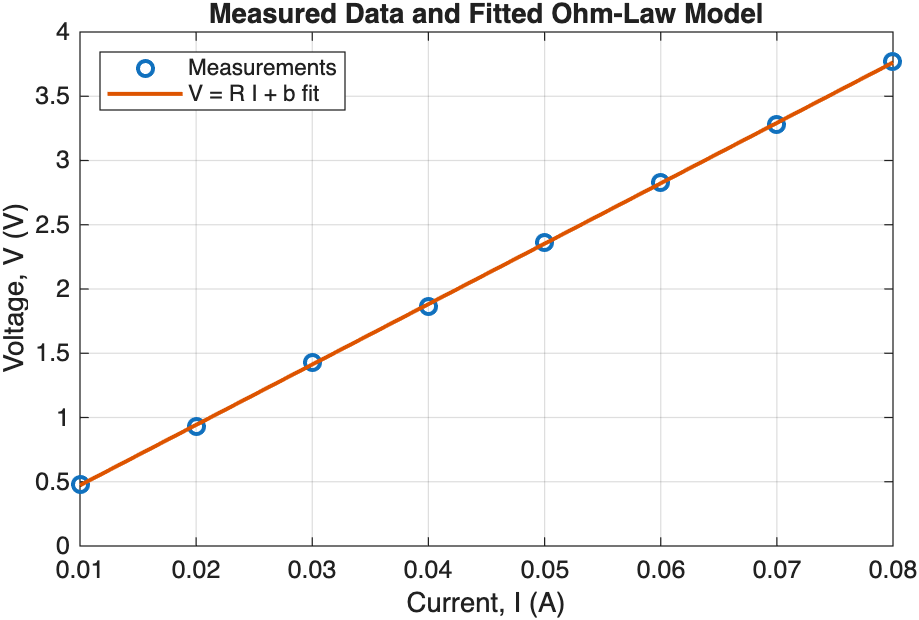
\includegraphics[width=.74\linewidth]{assets/week09_ohms_law_fit.png}
\caption{Locked MATLAB reference: measured voltage-current points and the fitted $V=RI+b$ model. The slope is $47.0000\,\Omega$.}
\end{figure}

An overlay is useful, but visual closeness alone is not enough. The next step asks where and by how much the model misses each measurement.

\section*{6. Residuals make model--data disagreement visible}
For measurement $i$, define
\[
r_i=V_{i,\mathrm{measured}}-V_{i,\mathrm{fit}}.
\]
A positive residual means the measured voltage is above the fitted line. A negative residual means it is below. Residuals have unit volts because they are voltage differences.

For the locked data, the residual root-mean-square value is about
\[
\mathrm{RMSE}_r=0.0130\units{V},
\]
and the largest absolute residual is $0.0225\units{V}$.

\begin{figure}[H]
\centering
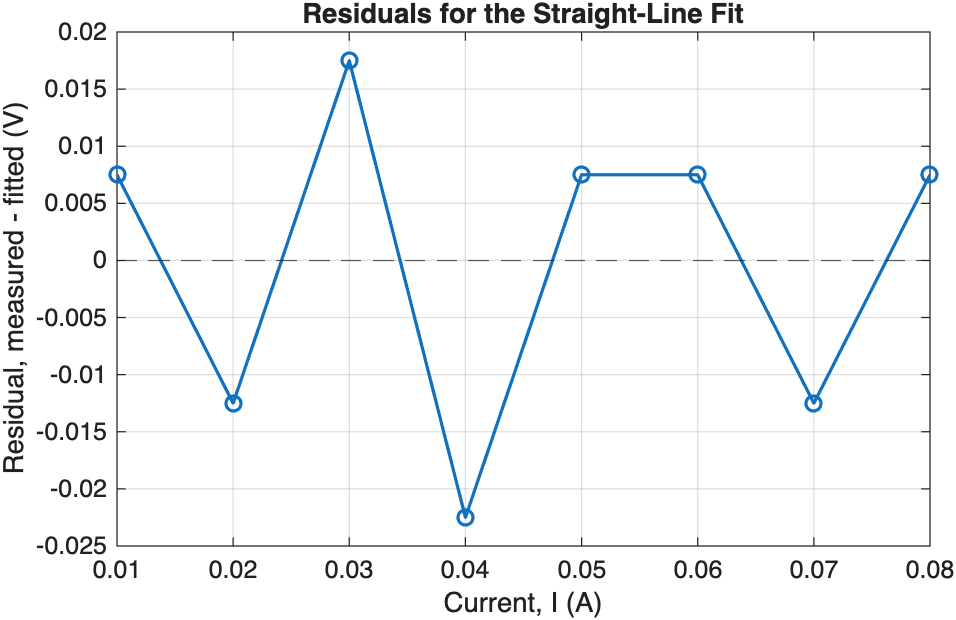
\includegraphics[width=.70\linewidth]{assets/week09_ohms_law_residuals.png}
\caption{Residuals alternate around zero and show no obvious curved pattern in this small dataset.}
\end{figure}

The absence of obvious structure supports the straight-line model \emph{over this measured range}. It does not prove that the resistor is perfectly ohmic at every current or temperature.

\begin{checkbox}\textbf{Core model-quality check.} Small residuals are not enough by themselves. Ask whether they show a pattern. A U-shaped sequence---positive at both ends and negative in the middle---would suggest missing curvature or another systematic effect.\end{checkbox}

\section*{7. Validate the fitted resistance with a physical reference}
The resistor is labelled $47\,\Omega$ with a nominal $5\%$ tolerance. The manufacturer range is therefore
\[
47(1-0.05)=44.65\,\Omega,
\qquad
47(1+0.05)=49.35\,\Omega.
\]
The fitted value $47.0000\,\Omega$ lies inside this range. This is an independent physical/reference check because the nominal component information did not come from the fitting calculation.

\begin{aibox}\textbf{Tolerance is not fit uncertainty.} The $5\%$ label describes the component specification. It does not tell us how much the fitted resistance would change if we repeated this measurement procedure. Keep these two ideas separate.\end{aibox}

\section*{8. State uncertainty only as strongly as the evidence allows}
Three supplied repeat runs give fitted slopes
\[
47.00,\quad47.06,\quad47.27\,\Omega.
\]
For Week 9, use the observed span as a simple repeatability range:
\[
47.0\text{ to }47.3\,\Omega.
\]
A defensible statement is:

\begin{keybox}\textbf{Cautious result.} The fitted resistance is about $47.1\,\Omega$, with repeat runs spanning roughly $47.0$--$47.3\,\Omega$ for this supplied measurement procedure. This range is not a formal confidence interval and does not include every possible systematic error.\end{keybox}

Notice the reporting precision. Writing $47.111111\,\Omega$ would imply more certainty than the repeated data support.

\section*{9. Worked reasoning chain}
Use the same chain whenever a familiar physical dataset is fitted:

\begin{center}\small
\begin{tabular}{p{.24\linewidth}p{.68\linewidth}}
\toprule
Step & Week 9 evidence\\
\midrule
Physical model & $V=RI+b$ for an approximately ohmic resistor\\
Variables and units & $I$ in A, $V$ and $b$ in V, $R$ in $\Omega$\\
Algorithm & plot $\rightarrow$ fit $\rightarrow$ predict $\rightarrow$ residuals $\rightarrow$ validate\\
Code & supplied \texttt{polyfit} and \texttt{polyval} scaffold\\
Error/uncertainty & residual scatter and repeat-run range\\
Validation & fitted $R$ inside the independent nominal component range\\
Interpretation & linear model is adequate over the supplied current range\\
\bottomrule
\end{tabular}
\end{center}

This sequence is more important than memorising a fitting function name. In an assessment, the syntax may be supplied; you still need to explain the physical parameter, unit, residual evidence, and justified conclusion.

\section*{Working exposure: one fit-quality statistic}
You may be shown a supplied coefficient of determination, $R^2$. Values closer to 1 indicate that the fitted predictions account for more of the observed variation in that dataset. Treat it as supporting evidence only. A high $R^2$ does not repair wrong units, a poor physical model, a structured residual pattern, or an unverified data-entry error.

You may also be shown two plausible simple models and their residual evidence. Compare the supplied evidence; independent reproduction of advanced selection metrics is not required.

\section*{Optional stretch}
Weighted fitting, nonlinear fitting, covariance matrices, regularisation, and formal confidence intervals are outside the Week 9 Core route. They are not required for ordinary pass-level work here.

\section*{Three takeaways}
\begin{enumerate}[nosep,leftmargin=7mm]
\item A fitted parameter must keep the unit implied by the physical equation.
\item Residuals show where the model misses the measurements; visible structure can reveal a poor model even when the overlay looks convincing.
\item Report uncertainty only to the level supported by the evidence, and keep repeatability distinct from manufacturer tolerance or formal confidence intervals.
\end{enumerate}

\begin{keybox}\textbf{Preparation for the practical.} Be ready to fit a supplied straight-line scaffold, state parameter units, read residual structure, use one independent check, and report uncertainty only to justified precision.\end{keybox}

\end{document}
